\subsection{Hydro-mechanical response of a single fracture within a rock matrix (2D)}

\subsubsection*{Definition}
This example is a fluid injection problem into a single discrete fracture surrounded by an impermeable rock matrix in two-dimensional space and validates the proposed lower-dimensional interface elements with local enrichments for the nonlinear, coupled HM problem. 
The test case is designed to mimic the semi-analytical similarity solution available in \cite{Wijesinghe1986}, which has been used to verify numerical codes such as ROCMAS II \cite{Noorishad1992}, GEOCRACK \cite{Swenson1995}, and FEHM \cite{Bower1997}. Test parameters are referred to those of  \cite{Bower1997}.
The solution is available based on the following assumptions:
\begin{enumerate}
\item  The fluid compressibility is small compared to the compliance of the fracture aperture under normal effective stress. (This is valid for liquid saturated fractures.)
\item  Fluid flow in a fracture is laminar flow between parallel surfaces.
\item  Fracture deformation is not hysteretic.
\item  The gradient in aperture along the fracture is small. There is no shear deformation of the fracture or the fracture does not dilate when sheared.
\item  Displacements parallel to the fracture are negligible everywhere within the rock mass.
\end{enumerate}

Figure \ref{fig:ex_hm_single_problem} shows a sketch of the calculation model. The major fracture lies horizontally in the middle of an impermeable rock block.  
The fracture is subjected to a uniform in-situ stress $\stress_{yy}=50$ MPa normal to the fracture. Initially, fracture aperture is uniformly $b_0 = 1.0 \cdot 10^{-2}$ mm and fluid pressure is $p_0=11.0$ MPa along the fracture. At time $t=0^+$, fluid is injected at the left-most edge of the fracture (in the form of constant boundary pressure, $p=11.9$ MPa) and a sudden increase of pressure in the fracture results.
%
The injection pressure induces elastic fracture opening and a subsequent increase of fracture permeability and storage capacity. 
%
\begin{figure}[!tbh]
\centering
\includegraphics[width=120mm]{chapter_14/figures/fig_14_4_26}
\caption{Fluid injection into a discrete fracture-rock matrix system.}
\label{fig:ex_hm_single_problem}
\end{figure}

\begin{table}[!htb]
\centering
\caption{Model parameters}
\label{tbl:ex_hm_single_setting}
\begin{tabular}{llrr}
\toprule
Symbol & Parameter & Value & Unit \\
\midrule
\multicolumn{4}{l}{\textit{Fluid}}  \\ 
$\rho^l$ & Density & 1000.0 & $kg \cdot m^{-3}$ \\  
$\mu$ & Viscosity & 0.001 & $Pa \cdot s$ \\  \\ 
\multicolumn{4}{l}{\textit{Porous medium}}  \\  
$\rho^s$ & Density & 2716.0 & $kg \cdot m^{-3}$ \\ 
$S_s$ & Specific storage & $1.0\cdot 10^{-10}$ & ${Pa}^{-1}$ \\ 
$k$ & Permeability & $1.0\cdot 10^{-21}$ & $ m^2 \cdot s^{-1}$ \\ 
$\phi$ & Porosity & 0.1  & $ \%$ \\ 
$E$ & Young's modulus & 60 & $ GPa$ \\ 
$\nu$ & Poisson ratio & 0.0 & $-$ \\ 
$\alpha$ & Biot constant & 1.0 & $-$ \\  \\
\multicolumn{4}{l}{\textit{Fracture}}  \\  
$b_0$ & Initial aperture & $1.0\cdot 10^{-5}$ & $m$ \\ 
$S_s$ & Specific storage & 0.0 & $Pa^{-1}$ \\ 
$k_n$ & Joint normal stiffness & 100 & $GPa \cdot m^{-1}$ \\ 
$k_s$ & Joint shear stiffness & 100 & $GPa \cdot m^{-1}$ \\ 
$\alpha$ & Biot constant & 1.0 & $-$ \\ 
\bottomrule
\end{tabular}
\end{table}

\subsubsection*{Semi-analytical solution}
Wijesinghe \cite{Wijesinghe1986} derived the ordinal differential equation with the dimensionless aperture $w$. The semi-analytical solution can be obtained by solving the equation as an initial value problem using the fourth order Runge-Kutta method. For details, please refer to the original work \cite{Wijesinghe1986}. %Initial values are $w1(0)$, $w2(0)$. However, $Q(0)$, which is used for $w1(0)$ is still unknown. Thus, an iterative method with changing $Q(0)$ needs to be executed to satisfy a boundary condition $w2( \infty )=1$. \cite{Wijesinghe1986} suggests using $w2(10)=1$.

\subsubsection*{Numerical solution}
Boundary fluid pressure is fixed at $t=0^+$ to 11.9 MPa at the left and 11 MPa at the right. Line elements with local enrichment were used to represent the discrete fracture and quadrilateral elements for surrounding rock matrix. Very fine vertical discretization is required near the fracture, i.e. $\Delta y$=0.001 m. The time step is selected as 10 s and a Newton-Raphson iteration is utilized to solve the nonlinear equation. 

\subsubsection*{Results}
Simulation results are presented in Figure \ref{fig:ex_hm_single_result} for pressure and fracture aperture profile along the fracture. When fluid is injected, the fracture aperture is instantaneously opened to nearly 1.9 $\cdot 10^{-2}$ mm at the injection point ($x = 0$ m). With time, this fracture opening behavior gradually propagates toward the right-most, low-pressure edge of the fracture. Linear constitutive laws dictate a linear variation in fracture aperture relative to fluid pressure.
%discussion
Figure \ref{fig:ex_hm_single_result} shows good agreement between the  numerical method and the semi-analytical solution.

\begin{figure}[!tbh]
\centering
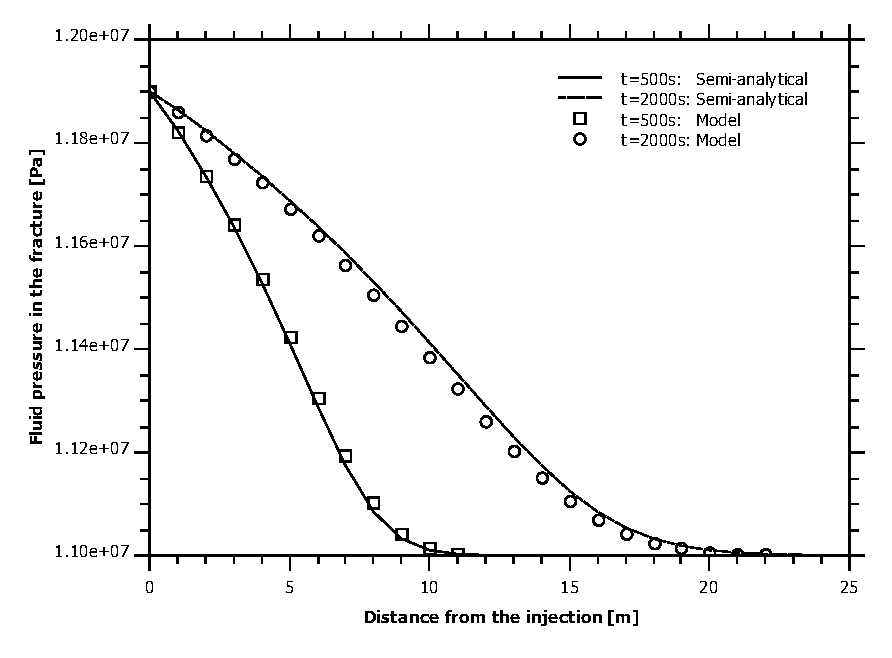
\includegraphics[width=100mm]{chapter_14/figures/fig_14_4_27_a}
\includegraphics[width=100mm]{chapter_14/figures/fig_14_4_27_b}
\caption{Profile along the fracture: pressure (left) and aperture (right).}
\label{fig:ex_hm_single_result}
\end{figure}
